\documentclass[article]{jss}

\usepackage{booktabs}
\usepackage{longtable}
\usepackage{array}
\usepackage{microtype}
\usepackage{url}
\usepackage{xspace}
\usepackage{float}

\newcommand{\fastEmbedR}{\pkg{fastEmbedR}\xspace}
\newcolumntype{L}[1]{>{\raggedright\arraybackslash}p{#1}}

\author{Moussa Kassim Mohamed$^{1,2,*}$ \quad Martin Ocharo$^{1,2,*}$\\
  Giulia Canarutto$^{3,4}$ \quad Dalia Ahmed$^1$ \quad Dupe Ojo$^1$\\
  Alessia Vignoli$^{5,6}$ \quad Leonardo Tenori$^{5,6,\dagger}$\\
  Dinesh Gupta$^{7}$ \quad Silvano Piazza$^{3,8}$\\
  Stefano Cacciatore$^{1,2,\dagger}$}

\title{\fastEmbedR: Multicore and GPU UMAP and
  Compact-Support t-SNE in \proglang{R}}

\Plaintitle{fastEmbedR: Multicore and GPU UMAP and
  Compact-Support t-SNE in R}
\Shorttitle{Multicore and GPU Embeddings in R}
\Plainauthor{Kassim, Ocharo, Canarutto, Ahmed, Ojo, Vignoli, Tenori, Gupta,
  Piazza, Cacciatore}

\Abstract{
  Uniform manifold approximation and projection (UMAP) and
  t-distributed stochastic neighbor embedding (t-SNE) are widely used
  for exploratory visualization, but large data sets make neighbor search,
  initialization, graph construction, and layout optimization expensive.
  \fastEmbedR is an MIT-licensed \proglang{R} package that implements fuzzy
  UMAP and a compact-support interpolation-based t-SNE variant, with candidate
  width equal to perplexity, on multicore CPU, Apple Metal, and NVIDIA CUDA.
  Matrix, float32, and reusable nearest-neighbor inputs share strict backend
  reporting. The package also provides randomized principal component
  analysis (PCA), reusable weighted graphs, community detection, optional
  landmark fitting, and fixed-reference projection.
  Component tests compare graph weights, affinities, forces, gradients, and
  trajectories with independent references. The benchmark design evaluates
  complete public calls separately from direct-Python fits and records
  runtime, memory, observed neighbor recall, and embedding quality. The
  available full-data, 11-data-set workflow campaign is diagnostic because
  its final audit failed. It does not establish release-level speedups. Source,
  documentation, and reproducible benchmark code are publicly available.
}

\Keywords{dimensionality reduction, GPU computing, Metal, CUDA, PCA,
  t-SNE, UMAP}
\Plainkeywords{dimensionality reduction, GPU computing, Metal, CUDA, PCA,
  t-SNE, UMAP}

\Address{
  $^1$Bioinformatics Unit, International Centre for Genetic Engineering and\\
  Biotechnology (ICGEB), Cape Town 7925, South Africa\\
  $^2$Department of Integrative Biomedical Sciences, Institute of Infectious
  Disease \& Molecular Medicine, University of Cape Town, Cape Town 7925,
  South Africa\\
  $^3$Computational Biology Group, International Centre for Genetic
  Engineering and Biotechnology (ICGEB), Trieste, Italy\\
  $^4$Life Science Department (DSV), University of Trieste, Trieste, Italy\\
  $^5$Department of Chemistry ``Ugo Schiff'', University of Florence,
  Sesto Fiorentino, Italy\\
  $^6$Magnetic Resonance Center, University of Florence,
  Sesto Fiorentino, Italy\\
  $^7$Translational Bioinformatics Group, ICGEB, New Delhi, India\\
  $^8$Bioinformatics Facility, Department of Cellular, Computational and
  Integrative Biology - CIBIO, University of Trento, Trento, Italy\\
  $^*$These authors contributed equally.\\
  $^\dagger$Co-corresponding authors:\\
  E-mail: \email{tenori@cerm.unifi.it},
  \email{stefano.cacciatore@icgeb.org}\\
  URL: \url{https://github.com/tkcaccia/fastEmbedR}
}

\begin{document}

\section{Introduction}

Uniform manifold approximation and projection (UMAP) and t-distributed
stochastic neighbor embedding (t-SNE) are standard tools for inspecting
high-dimensional data in genomics, cytometry, image analysis, and machine
learning \citep{vandermaaten2008,mcinnes2018,kobak2019}. Their output is a
low-dimensional layout that aims to retain local relationships from the
original feature space. The computational burden is not limited to the final
optimization. A complete workflow also includes preprocessing,
$k$-nearest-neighbor (KNN)
search, graph or affinity construction, initialization, and data movement
between the \proglang{R} process and an accelerator.

Several implementations address individual parts of this problem.
Barnes-Hut t-SNE reduces repulsive-force complexity
\citep{vandermaaten2014}; interpolation-based t-SNE uses a regular grid and
fast Fourier transform (FFT) convolutions \citep{linderman2019}; and GPU
implementations accelerate both t-SNE and UMAP
\citep{chan2018,nolet2020}. In \proglang{R}, \pkg{Rtsne} and \pkg{uwot}
provide mature CPU workflows, while FIt-SNE, Python openTSNE, umap-learn, and
RAPIDS cuML provide additional CPU or CUDA routes. A user nevertheless often
has to combine several packages or language environments, materialize the
same neighbor graph repeatedly, and accept different data types and timing
boundaries.

\fastEmbedR addresses this systems problem with one native \proglang{R}
interface for multicore central processing units (CPUs), Apple Metal, and
NVIDIA Compute Unified Device Architecture (CUDA). Its principal contributions
are software-engineering rather than new UMAP or t-SNE mathematics:
\begin{itemize}
  \item package-owned float32 fuzzy UMAP and compact-support t-SNE
    implementations, including interpolation-based repulsion, with strict
    backend reporting;
  \item matrix and precomputed-neighbor interfaces that reuse native
    nearest-neighbor results and avoid unnecessary host-device transfers;
  \item landmark models and fixed-reference transformation for new samples;
  \item shared CPU, Metal, and CUDA validation tests for affinities, graph
    weights, forces, optimization, precision, and difficult inputs; and
  \item typed results carrying resolved parameters, precision, backend, and
    timing information.
\end{itemize}

Supporting utilities provide backend-native randomized PCA for preprocessing
and t-SNE initialization and native weighted graph construction with Louvain,
Leiden, and Walktrap community detection. These utilities complete common
embedding workflows but are not the basis of the principal embedding claims.

The package is intentionally not an API clone of any one reference
implementation. It follows the published UMAP objective and the
interpolation-based t-SNE optimizer, while its production t-SNE affinity uses
compact support with one non-self candidate neighbor per unit of perplexity.
This policy differs from conventional sparse t-SNE workflows with wider
candidate sets. Fuzzy UMAP is the default. A binary graph mode
is retained as a separately labeled adjacency sensitivity analysis that can
emphasize cluster boundaries, but it changes the graph objective and is not a
replacement for standard fuzzy UMAP.

Table~\ref{tab:related-software} summarizes capabilities of the listed
versions. Multicore CPU indicates user-selectable parallel CPU work; KNN
input means that an embedding can consume precomputed nearest neighbors.
For landmarking, ``manual'' means fitting a selected reference subset and
projecting the remainder through a separate public transform method,
whereas ``built-in'' includes landmark selection and projection.

\begin{table}[t]
\centering
\caption{Core embedding capabilities of related software. Experimental
  file-backed routes are excluded.}
\label{tab:related-software}
\footnotesize
\renewcommand{\arraystretch}{1.15}
\setlength{\tabcolsep}{3pt}
\begin{tabular}{L{0.22\textwidth}L{0.09\textwidth}ccc
                L{0.13\textwidth}L{0.09\textwidth}L{0.09\textwidth}}
\toprule
Software & Method & Multi-CPU & CUDA & Metal & Landmarking &
  KNN input & 3D output \\
\midrule
\pkg{Rtsne} 0.17 & t-SNE & Yes & No & No & No & Yes & Yes / -- \\
FIt-SNE 47ff14f & t-SNE & Yes & No & No & No & Limited & Yes / -- \\
openTSNE 1.0.4 & t-SNE & Yes & No & No & Manual & Yes & Yes / -- \\
\pkg{uwot} 0.2.5 & UMAP & Yes & No & No & Manual & Yes & -- / Yes \\
\pkg{umap} 0.2.10.0 & UMAP & No & No & No & Manual & Yes & -- / Yes \\
umap-learn 0.5.12 & UMAP & Yes & No & No & Manual & Yes & -- / Yes \\
RAPIDS cuML 26.06 & UMAP, t-SNE & No & Yes & No & UMAP only &
  Yes & No / Yes \\
\fastEmbedR & UMAP, t-SNE & Yes & Yes & Yes & Built-in & Yes &
  Yes / Yes \\
\bottomrule
\end{tabular}
\par\smallskip
\parbox{0.98\textwidth}{\scriptsize The 3D column is ordered t-SNE / UMAP;
  a dash means the method is not implemented. FIt-SNE and openTSNE use a
  Barnes--Hut route for 3D output rather than FFT interpolation. cuML's
  3D output and reference projection are UMAP-only. fastEmbedR supports
  three-dimensional t-SNE and UMAP on CPU, CUDA, and Metal
  for ordinary matrix or precomputed-neighbor fits. Three-dimensional GPU
  landmark refinement and full-graph CUDA t-SNE are not available.}
\end{table}

This article combines the software description, implementation details,
usage examples, numerical validation, workflow benchmarks, and limitations.
UMAP and t-SNE remain the central embedding contribution; PCA and graph
clustering are evaluated as integrated computational stages that let an
analysis remain within the same typed, backend-aware workflow.

\section{Software architecture}

\subsection{Execution model and ownership boundary}

The principal execution path begins with a matrix that may be centered,
scaled, or reduced by randomized PCA. Nearest-neighbor search
provides the sparse local relationships required by both methods. UMAP turns
these relationships into a weighted graph; t-SNE turns them into sparse
probabilities. A backend-specific optimizer then produces the final layout.
Precomputed neighbors can enter after the search stage, and landmark models
separate reference fitting from projection of omitted or genuinely new rows.

The required R layer is limited to \pkg{Rcpp}, \pkg{withr}, and the
\pkg{methods} package distributed with R; only \pkg{Rcpp} is a compiled-code
linking dependency. The CPU native core otherwise requires a C++17 toolchain
and the Basic Linear Algebra Subprograms (BLAS), Linear Algebra Package
(LAPACK), and Fortran runtime already configured for R. Matrix workflows use
the package's native neighbor layer, whereas the precomputed-neighbor
interfaces define an explicit boundary at which a caller can supply indices
and distances. The selected metric, neighborhood size, search engine,
observed recall, and backend are retained for reproducibility. Search time
remains part of complete public-workflow timing.
A comparative study of nearest-neighbor algorithms is outside the scope of
this article, but the accuracy of the search used by each reported workflow is
measured because it can affect both runtime and embedding quality. Metal and
CUDA builds link optional accelerator libraries; they do
not redistribute them. Copyright and third-party notices are retained in the
package source.

Explicit backend requests are strict. If \code{backend = "metal"} or
\code{backend = "cuda"} is unavailable, the function raises an error instead
of silently reporting CPU work as accelerated work. When \code{backend = NULL},
the session option and environment-variable policy are consulted, with CPU as
the final default. Successful results record both the requested and observed
backend; unavailable accelerator requests fail before a result is returned.

\subsection{Data representation and memory}

The production numerical payload uses float32. Ordinary \proglang{R} matrices
require one controlled conversion at the native boundary. Objects from
\pkg{float} are read directly. Neighbor distances, affinities, graph weights,
layouts, gradients, gains, and update buffers remain float32; indices and
compressed sparse row (CSR) offsets use int32. A float32 input returns a
float32 layout, whereas an ordinary matrix returns a double matrix only at the
final \proglang{R} boundary.

The memory reduction is smaller than 50 percent in a complete process because
object headers, labels, int32 graph structure, search indexes, FFT padding,
spectra, and allocator workspaces are not double-precision payloads. CUDA keeps
eligible neighbor, graph, affinity, layout, and optimizer buffers on-device.
Metal uses unified memory, so separate host and device peaks cannot be added
meaningfully. The result records persistent and temporary native-buffer
estimates when available.

\subsection{Experimental file-backed workflows}

The ordinary matrix interfaces remain the default. For an explicit
file-backed analysis, \code{massive_matrix()} describes a row-major float32
\code{.f32} or \code{.fbin} file without reading all observations into R.
The same \code{pca()}, \code{umap()}, and \code{tsne()} entry points accept
this descriptor with a selected \code{massive} mode and persistent output
path. Streamed PCA reads bounded row blocks and writes scores to disk.
The \code{landmark} embedding mode fits selected reference rows and
projects the others; this is an approximation to fitting every row, even
though the output contains coordinates for every observation. Neither
UMAP nor t-SNE automatically selects this approximation in response to
memory pressure.

A separate \code{out\_of\_core\_graph} mode consumes a prepared file-backed
fuzzy graph for UMAP or affinity graph for t-SNE, together with initial
coordinates. Graph construction can use the package's existing CPU
exact/HNSW or CUDA cuVS exact/IVF search routes. Thus, file-backed
optimization of all rows is distinct from landmark projection, but it
does not imply exact nearest-neighbor search. The full path currently
requires explicit preparation of its graph and initialization; a single
file-to-layout call is not claimed. CPU and CUDA stages have been exercised
experimentally, while Metal file-backed processing is unavailable and
raises an error. Selected CUDA PCA, search, and projection stages can
partition rows across devices; the complete embedding optimizer is not
distributed across GPUs. Memory budgets constrain algorithm buffers,
not total process resident memory or disk-cache use.

\subsection{Public interface}

Table~\ref{tab:api} maps the stable interface. Generic names are always shown
with namespace qualification in mixed-package sessions, for example
\code{fastEmbedR::umap()} and \code{fastEmbedR::pca()}.

\begin{table}[t]
\centering
\caption{Canonical public API. CPU, Metal, and CUDA are available where the
  package was compiled with the corresponding backend.}
\label{tab:api}
\scriptsize
\begin{tabular}{>{\raggedright\arraybackslash}p{0.31\textwidth}
  >{\raggedright\arraybackslash}p{0.52\textwidth}}
\toprule
Function & Purpose \\
\midrule
\code{tsne()}, \code{umap()} & Complete
  matrix-to-layout workflows. \\
\code{tsne_knn()}, \code{umap_knn()} & Layout from
  reusable neighbor indices
  and distances. \\
\code{precompute_knn()} & Backend-native non-self neighbor search. \\
\code{pca()} & Randomized PCA and optional t-SNE-scaled initialization. \\
\code{select_landmarks()} & Reusable landmark/reference selection. \\
\code{project_landmark_}\allowbreak\code{model()} & Project omitted or new observations into a
  fixed reference. \\
\code{transform_tsne()} & Fixed-reference t-SNE transformation. \\
\code{knn_graph()}, \code{graph_cluster()} & Secondary graph construction and
  Louvain, Leiden, or Walktrap clustering. \\
\bottomrule
\end{tabular}
\end{table}

The principal embedding functions return an S3
\code{fastEmbedR_embedding} object with coordinates, resolved parameters,
requested and observed backend, precision, stage timings, and optional neighbor
state. Methods for \code{print()} and \code{plot()} provide concise summaries.
Neighbor, PCA, landmark, graph, and clustering results have dedicated classes.
The current source accepts three-dimensional t-SNE and fuzzy UMAP on CPU,
CUDA, and Metal for ordinary fits. The evaluated image predates native 3D
GPU support, so its benchmarks do not validate those newer routes.

\section{Algorithms and backend implementations}

\subsection{UMAP}

UMAP constructs a fuzzy graph from local distances and optimizes a
low-dimensional cross-entropy objective \citep{mcinnes2018}. For observation
$i$, the package estimates local connectivity $\rho_i$ and scale $\sigma_i$,
forms directed membership strengths, and combines reciprocal memberships as
\[
  w_{ij} + w_{ji} - w_{ij}w_{ji}.
\]
The resulting CSR graph stores the row pointer, column index, weight, and edge
sampling schedule once. Fuzzy weighting is the standard default. Binary mode
sets unit weight on the symmetric neighbor union; it can make adjacency-defined
boundaries visually sharper, but it changes the objective and its quality
varies by data set.

The CPU optimizer uses contiguous arrays, thread-local random-number streams,
and atomic updates. The Metal implementation retains graph, coordinates, and
optimizer state in unified memory. CUDA consumes a resident nearest-neighbor
object, constructs the graph on-device, uses pooled memory for temporary
storage, and groups rows for coalesced access. Its production row optimizer
assigns one warp to a head row, fuses attraction, negative sampling,
repulsion, and coordinate updates, and aggregates the head update before
issuing tail atomics. Negative samples are generated on-device from the
per-edge epoch state. Repeated epoch work is captured as a CUDA Graph while
the graph, layout, and optimizer buffers are reused. The package owns the
optimizer policy and records the resolved values. The public controls are
neighborhood size, metric, fuzzy or binary graph mode, preprocessing, backend,
seed, output dimension, and CPU cores. The number of epochs, learning rate,
minimum distance, spread, repulsion strength, and negative-sample rate are
fixed internally by the recorded release policy.

\subsection{Compact-support interpolation-based t-SNE}

t-SNE converts local high-dimensional distances into probabilities $p_{ij}$
and minimizes Kullback-Leibler (KL) divergence from these probabilities to the
low-dimensional Student distribution \citep{vandermaaten2008}. \fastEmbedR
implements sparse Gaussian affinity construction, early exaggeration,
momentum, adaptive gains, gradient clipping, and interpolation-based FFT
repulsion for two-dimensional layouts in the evaluated image
\citep{linderman2019}.

The package uses compact affinity support: perplexity $P$ selects
$\lceil P \rceil$ non-self candidate neighbors. This policy is shared by the
matrix, precomputed-neighbor, landmark, and transformation interfaces and by
the CPU, Metal, and CUDA backends. The candidate width, achieved perplexity,
optimizer schedule, learning rate, exaggeration, and repulsion method are
returned with the fit.
For a conditional probability vector over $k$ candidates,
$H(p_i) \leq \log(k)$. Consequently, when $k=P$, the target entropy
$\log(P)$ lies at the boundary and is attained exactly only by uniform
conditional weights. The finite solver tolerance produces nearly uniform,
rather than mathematically identical, weights. High-dimensional distances
therefore determine candidate membership much more strongly than relative
mass within a candidate row; reciprocity during symmetrization can still
differentiate the final undirected edge weights.
The production API does not expose a wider affinity-support mode; therefore,
all cross-backend t-SNE validation in this article evaluates this same compact
policy, including the CUDA backend.

The FFT grid is selected by observation count $n$, with each reported size
denoting cells per coordinate axis. For two-dimensional layouts, CPU uses
128 cells for $n<40{,}000$ and 256 otherwise; Metal uses 128 for
$n<10{,}000$ and 256 otherwise; CUDA uses 256 for $n<20{,}000$,
512 for $20{,}000\leq n<100{,}000$, and 1024 otherwise. The
\code{FASTEMBEDR_TSNE_FFT_GRID} environment variable can override the
two-dimensional choice: CPU and Metal round a positive request up to a
power of two within 32--512, whereas CUDA accepts only powers of two
from 32 through 1024. FFT convolution pads each axis to twice the
selected grid size. UMAP does not use this repulsion grid. The evaluated
container does not provide native three-dimensional accelerator fits;
three-dimensional claims require a new image and separate validation.

Grid resolution is not a common tunable parameter across implementations.
The tested cuML 26.6.0 t-SNE fixes three interpolation points and 50
intervals per axis in its FFT source; its Python API offers no grid control.
FIt-SNE exposes the interpolation order and minimum interval count, but its
effective grid can increase with coordinate span. The updated benchmark
requests a FIt-SNE lower bound close to the CPU grid and records both
policies. Neither setting makes the grids identical, and these changes were
not applied to the diagnostic campaign reported below.

CPU execution retains FFT plans, grids, and thread scratch across iterations.
Metal uses native grid deposition, FFT, interpolation, and update kernels.
CUDA retains cuFFT plans, workspaces, coordinates, gains, updates, and force
buffers and uses CUDA Graph execution for repeated iteration groups. Device
synchronization occurs before a public function returns, so elapsed time does
not omit queued accelerator work. On CUDA, the layout-statistics, grid
deposition, batched spectral products, interpolation, attractive-force, and
optimizer-update stages are encoded in the captured iteration sequence. The
global mean reduction and final centering remain separate kernels because they
require completed cross-block reductions; keeping this dependency explicit
preserves the objective and update order while avoiding host-side launches.

\subsection{PCA and initialization}

Randomized singular value decomposition approximates a low-rank subspace using
random projection and power iterations \citep{halko2011}. The public
\code{fastEmbedR::pca()} function returns scores, loadings, singular values,
centering and scaling vectors, decomposition metadata, and the observed
backend. With
\code{tsne_init = TRUE}, it also centers the requested low-dimensional scores
and rescales them so that the largest component standard deviation is
$10^{-4}$, which is directly accepted by \code{fastEmbedR::tsne()} and
\code{fastEmbedR::tsne_knn()}.

CPU PCA uses a blocked float32 randomized range finder followed by a small
dense decomposition. Metal uses a float32 block-subspace randomized
decomposition with Metal Performance Shaders. CUDA selects between native
float32 randomized SVD and resident RAPIDS RAFT truncated singular value
decomposition from matrix shape, requested rank, and estimated arithmetic
cost. The typed result includes scores,
loadings, singular values, preprocessing vectors, optional test-set
projections, and the observed backend. Comparisons with \pkg{irlba}
\citep{irlba2026} assess performance and agreement between two approximate
methods rather than treating either as an exact reference.
The PCA alignment study evaluates CPU, the tested M3 Metal system, and CUDA.
Agreement is measured after Procrustes or subspace alignment because truncated
decompositions can return equivalent bases with different signs or rotations.
When PCA is requested inside an embedding workflow, its preprocessing and
transfer costs belong to the complete-call time; a standalone PCA benchmark
is reported separately. The shape-dependent CUDA choice is recorded for each
fit, because a faster truncated decomposition on one matrix shape need not
remain faster on another.

\subsection{Landmarks and new observations}

Landmarking is explicit. A reference subset is selected by a seeded
projection-diversity policy or supplied by the user. The ordinary
\code{fastEmbedR::tsne()} or \code{fastEmbedR::umap()} implementation embeds
that subset. Remaining
rows query the fixed reference, receive weighted or affine-interpolated
coordinates, and can undergo a short row-restricted refinement while reference
coordinates are restored after each update.

The package distinguishes reconstruction of omitted rows from prediction of
genuinely unseen observations. In held-out transformation, query rows do not
participate in landmark selection, reference preprocessing, neighbor search
among reference rows, initialization, or stopping. t-SNE query probabilities
are optimized with the reference fixed \citep{policar2021}; UMAP projects
queries through reference neighbors and optional fixed-reference refinement.
The returned model records landmark indices, preprocessing, neighborhood
policy, graph or affinity policy, backend, and stage timings. Landmarking is a
scalability approximation, not a guarantee of faster execution or unchanged
quality.

\subsection{Graph construction and community detection}

The same sparse-neighbor infrastructure constructs undirected weighted graphs
from a feature matrix or reusable KNN object. Edge weights can encode
shared-neighbor Jaccard similarity, inverse distance, or binary adjacency;
mutual-neighbor filtering and weight pruning alter the resulting graph and
must be reported with it. Reusing a graph permits community analyses without
another neighbor search, although graph construction remains a distinct
timed stage.

Package-native Louvain and Leiden support CPU, Metal, and CUDA local
movement, while exact Walktrap is CPU-only
\citep{blondel2008,traag2019,pons2006}. A clustering fit reports membership,
modularity, connectivity diagnostics, backend, and run parameters. Agreement
with \pkg{igraph} is assessed on the identical stored weighted graph, with
adjusted Rand index (ARI) for membership; stochastic algorithms need not
return identical partitions. These utilities support interpretation after
embedding but are not evidence for UMAP or t-SNE correctness.

\section{Using fastEmbedR}

\subsection{Installation and backend inspection}

A portable CPU installation requires \proglang{R}, \pkg{Rcpp}, \pkg{withr},
a C++17 compiler, and R's configured linear-algebra libraries. Metal
acceleration requires Apple Silicon, macOS 14 or later, Xcode 15 or later,
and the Foundation, Accelerate, Metal, Metal Performance Shaders, and Metal
Performance Shaders Graph frameworks supplied by the Apple software
development kit (SDK); these are not separate R-package dependencies.

CUDA acceleration requires an existing compatible NVIDIA driver and a
separately installed CUDA toolkit providing the CUDA runtime, cuFFT, cuBLAS,
cuSOLVER, and cuRAND. RAPIDS cuVS is required only when a CUDA workflow must
construct nearest neighbors directly from a matrix. CUDA embedding from a
precomputed-neighbor object does not require cuVS. RAPIDS RAFT and the RAPIDS
Memory Manager (RMM) are optional and are used only by the RAFT truncated
singular value decomposition branch of automatic CUDA PCA. The package no
longer links or loads FAISS; its retained FAISS notices document provenance
of adapted native algorithms rather than a runtime dependency.

The installation guide gives release-tested commands for a portable CPU
source build, an Apple Silicon Metal build with an explicit SDK, and a strict
CUDA build that fails when any requested CUDA, cuVS, or RAFT component is
missing. The suggested R packages are confined to optional float32 input,
validation, diagnostics, thread control, tests, and vignette construction;
they do not enlarge the minimum CPU runtime. A source install from an
immutable release tag is recommended for a publication analysis. The
accompanying replication script requests only the CPU backend and runs with
one core, so it also exercises the minimum installation.

Session defaults are set with \code{options(backend = "cuda")} and
\code{options(n.cores = 4L)}. An explicit function argument takes precedence;
the environment variable \code{FASTEMBEDR_BACKEND} is consulted only when no
explicit argument or session option is present. CPU remains the final default.
The requested and observed backends are recorded in each successful result,
and an unavailable explicit accelerator request raises an error. Tested
examples are maintained in the package vignette and online tutorial.

The benchmark preflight executes this CPU example:
\begin{verbatim}
set.seed(4)
x <- matrix(rnorm(128 * 8), 128, 8)
options(backend = "cpu", n.cores = 2L)
fit <- fastEmbedR::umap(x, n_neighbors = 15, seed = 4)
knn <- fastEmbedR::precompute_knn(x, k = 15)
from_knn <- fastEmbedR::umap_knn(
    knn$indices, knn$distances, seed = 4)
\end{verbatim}
The matrix fit returns \code{fit\$layout}; \code{from_knn} is a
two-column layout computed from the reusable neighbor result. An explicit
\code{backend} argument can override the session default.

\subsection{Matrix and precomputed-neighbor workflows}

The matrix interfaces \code{tsne()} and \code{umap()} perform preprocessing,
neighbor search, initialization, and optimization. The corresponding
\code{tsne_knn()} and \code{umap_knn()} interfaces consume reusable indices
and distances, avoiding repeated search in seed, optimizer, or graph-mode
comparisons. The CUDA route can retain the neighbor object on the device and
consume it directly during affinity or graph construction.

\subsection{PCA and landmark models}

The \code{pca()} interface returns ordinary scores and, with
\code{tsne_init = TRUE}, a scaled t-SNE initialization. Landmarking is enabled
within \code{tsne()} or \code{umap()} by supplying a fraction, count, or row
indices to \code{landmarks}; the default \code{FALSE} fits all observations.
The fitted result contains a reusable model accepted by
\code{project_landmark_model()} for independently held-out rows. Reference
coordinates remain immutable during projection.

With file-backed input, \code{pca()} streams scores when \code{massive}
is \code{out\_of\_core}. Setting \code{massive} to \code{landmark} in
\code{umap()} or \code{tsne()} fits a chosen reference subset and writes
projected coordinates to disk. The prepared-graph modes instead update
all observations. The experimental vignette documents file layout,
memory controls, checkpointing, and unsupported backend combinations.

\section{Validation}

\subsection{Validation strategy}

Final t-SNE coordinates are non-convex and need not be identical across
parallel implementations. Correctness was therefore tested below the final
layout as well as at the layout level. Tests used exact high-dimensional
neighbors and common initial coordinates where the compared APIs permitted
them. UMAP validation compared edge sets, fuzzy weights, aligned coordinates,
and embedding neighborhoods. t-SNE validation compared conditional and
symmetrized affinities, exact attractive and repulsive forces, finite-difference
gradients, FFT-grid force convergence, one-step updates, objective trajectories,
final KL divergence, aligned coordinates, and embedding neighborhoods.

PCA tests compare aligned scores, principal angles, captured variance, and
test-set projection. Graph tests use canonical clique graphs, stochastic block
models, isolated vertices, disconnected candidate communities, high-degree
vertices, and fixed real-data graphs. Louvain and Leiden are compared with
\pkg{igraph} modularity and membership; Walktrap is compared with the
\pkg{igraph} Pons--Latapy implementation.

Pathological embedding tests included duplicated observations, zero distances,
disconnected graphs, coincident coordinates, extreme finite coordinates, and
nonfinite input. CPU float32 forces were also compared with an independent
float64 oracle. Fixed seeds make the deterministic one-thread CPU route
repeatable, but do not guarantee bitwise Metal or CUDA identity because atomic
update order can differ.

\subsection{Affinity, graph, and force agreement}

On a fixed 2,000-point MNIST subset, fuzzy UMAP edge Jaccard agreement with a
\pkg{uwot} similarity graph was 1.000000; weight Pearson and Spearman
correlations were 0.999990 and 0.999977. On common compact t-SNE support,
edge Jaccard and Pearson weight agreement with Python openTSNE were 1.000000.
The Spearman value of 0.852 arose from rank changes among numerical near-ties:
all matched weights differed by less than $10^{-7}$ and the maximum absolute
difference was $1.66\times10^{-8}$. This validates arithmetic on the supplied
compact support, rather than equivalence to a conventional wider-support
t-SNE affinity model.

The fixed-input affinity characterization confirms the mathematical
consequence of this policy. At each tested perplexity, the achieved
perplexity equaled the supplied support width, normalized entropy was 1, and
the conditional coefficient of variation was numerically zero. Distances
therefore select the neighbors, while reciprocity in symmetrization provides
most of the remaining edge-weight variation. This is a deliberate compact
approximation and is not presented as affinity-equivalent to conventional
wider-support t-SNE.

Table~\ref{tab:numerical} reports lower-level t-SNE tests. FFT force error fell
from $5.07\times10^{-4}$ at grid 32 to $7.68\times10^{-6}$ at grid 256.
The CUDA validation exercises the production FFT path; it does not report an
unsupported exact-repulsion CUDA route as a passing test.

\begin{table}[t]
\centering
\caption{Component-level t-SNE validation. Relative L2 error is measured
  against the stated independent reference.}
\label{tab:numerical}
\scriptsize
\begin{tabular}{p{0.40\textwidth}p{0.21\textwidth}p{0.20\textwidth}}
\toprule
Component & Acceptance threshold & Maximum observed \\
\midrule
Float32 affinity versus float64 & $2\times10^{-6}$ absolute &
  $2.06\times10^{-8}$ \\
Exact attractive force & $5\times10^{-5}$ relative &
  $4.12\times10^{-7}$ \\
Exact repulsive force & $5\times10^{-5}$ relative &
  $1.68\times10^{-7}$ \\
Finite-difference gradient & $2\times10^{-4}$ relative &
  $1.27\times10^{-7}$ \\
FFT repulsion, grid 128 & $10^{-3}$ relative & $3.37\times10^{-5}$ \\
CPU-CUDA FFT first step & $2\times10^{-3}$ relative &
  $3.80\times10^{-8}$ \\
Common-affinity KL & $2\times10^{-5}$ absolute &
  $1.21\times10^{-6}$ \\
Pathological inputs & finite result or explicit error & 15 of 15 passed \\
\bottomrule
\end{tabular}
\end{table}

\subsection{Final-layout agreement}

Compact-support validation used common initialization and affinities for
2,000 observations from Fashion-MNIST, MNIST, MetRef, and USPS. The archived
1,000-normal-iteration outputs used seed 42 and a 256-cell FFT grid in
Table~\ref{tab:tsne-final-layout}. Other seed runs stopped at 750 normal
iterations; they cannot be counted as 1,000-iteration replications. The
corrected benchmark schedules seeds 4, 17, and 42 at 1,000 normal iterations
on the same grid. Until that run is complete, the table is a diagnostic
single-seed comparison, not evidence of between-seed stability. Metal was not
part of this Linux experiment and is not inferred from it.

\begin{table}[t]
\centering
\caption{Fixed-input compact-support t-SNE final-layout validation.
  Seed-42 diagnostic values at 1,000 normal iterations and a fixed 256-cell
  FFT grid. Python openTSNE supplies the common reference fit. USPS
  trustworthiness was present in the saved results.}
\label{tab:tsne-final-layout}
\scriptsize
\begin{tabular}{llrrr}
\toprule
Data set & Implementation & Common KL & Trustworthiness & Preserve@30 \\
\midrule
Fashion-MNIST & Python openTSNE & 1.2842 & 0.9819 & 0.5765 \\
 & \fastEmbedR CPU & 1.2835 & 0.9818 & 0.5784 \\
 & \fastEmbedR CUDA & 1.2829 & 0.9819 & 0.5783 \\
MNIST & Python openTSNE & 1.7367 & 0.9557 & 0.5228 \\
 & \fastEmbedR CPU & 1.7403 & 0.9539 & 0.5211 \\
 & \fastEmbedR CUDA & 1.7373 & 0.9557 & 0.5210 \\
MetRef & Python openTSNE & 1.8354 & 0.8460 & 0.4352 \\
 & \fastEmbedR CPU & 1.8476 & 0.8558 & 0.4427 \\
 & \fastEmbedR CUDA & 1.8378 & 0.8528 & 0.4405 \\
USPS & Python openTSNE & 1.6906 & 0.9577 & 0.5203 \\
 & \fastEmbedR CPU & 1.6889 & 0.9578 & 0.5229 \\
 & \fastEmbedR CUDA & 1.6900 & 0.9580 & 0.5218 \\
\bottomrule
\end{tabular}
\end{table}

Across three FFT grid sizes at seed 42 and 1,000 iterations, median
Procrustes correlations with Python openTSNE were
0.998, 0.930, 0.778, and 0.995 for CPU on Fashion-MNIST, MNIST, MetRef, and
USPS; the corresponding CUDA values were 0.998, 0.939, 0.764, and 0.992.
Neighborhood agreement at 30 ranged from 0.672 to 0.936 for CPU and from
0.650 to 0.935 for CUDA. The lower coordinate agreement on MetRef coexisted
with closely matched KL and local-neighborhood quality, illustrating why
non-convex t-SNE validation cannot rely on coordinate correlation alone.

With common precomputed neighbors and matched seeds, fixed-input UMAP
CPU-CUDA Procrustes correlation had median 0.962 across 33 data-set--seed
pairs (range 0.776--0.996). Neighborhood agreement at 30 had median 0.812
(range 0.473--0.900). The lowest agreements occurred for ImageNet and USPS;
their data-set medians were 0.904/0.474 and 0.799/0.574 for
Procrustes/neighborhood agreement. These results establish behavioral
agreement rather than bitwise identity and retain the weaker cases instead of
reporting only aggregate medians.

\subsection{Precision boundary}

Using the same exact neighbors, initialization, and seed, ordinary double
matrices and direct \pkg{float} inputs produced identical affinity or graph
weights, aligned layouts, neighborhood metrics, and t-SNE KL in the focused
boundary test. Runtime differences were small and not consistent across
objectives. The result supports numerical agreement and copy avoidance, not a
universal speedup for the float32 input class.

\section{Benchmark design}
\label{sec:benchmark}

\subsection{Data sets and hardware}

The diagnostic workflow campaign covered 11 external data sets
(Table~\ref{tab:data}):
image data, metabolomics, cytometry, single-cell RNA sequencing, and
foundation-model image features. No benchmark matrix or label vector is
distributed with the package. The package vignette uses only
\code{datasets::iris}.

\begin{table}[t]
\centering
\caption{Benchmark data sets and fitted row counts in workflow campaign
  \texttt{20260930T203319Z}. All rows were fitted. ImageNet features are
  used primarily as a
  scalability and memory stress test rather than a two-dimensional
  class-separation task.}
\label{tab:data}
\scriptsize
\begin{tabular}{lrrrl}
\toprule
Data set & Source rows & Fitted rows & Variables & Domain \\
\midrule
COIL20 & 1,440 & 1,440 & 16,384 & Object images \\
USPS & 11,000 & 11,000 & 256 & Handwritten digits \\
MNIST & 70,000 & 70,000 & 784 & Handwritten digits \\
Fashion-MNIST & 70,000 & 70,000 & 784 & Clothing images \\
MetRef & 873 & 873 & 375 & Metabolomics \\
mass41 & 965,282 & 965,282 & 14 & Mass cytometry \\
flow18 & 1,000,021 & 1,000,021 & 11 & Flow cytometry \\
ImageNet features & 1,281,167 & 1,281,167 & 1,024 & DINOv2 features \\
FlowRepository & 5,220,347 & 5,220,347 & 32 & Mass cytometry \\
Tabula Muris & 100,102 & 100,102 & 50 & Single-cell RNA-seq PCs \\
Macosko retina & 44,808 & 44,808 & 50 & Single-cell RNA-seq PCs \\
\bottomrule
\end{tabular}
\end{table}

Linux CPU and CUDA jobs ran on the University of Cape Town high-performance
computing facility. CPU nodes used Intel Xeon Gold 6442Y processors; the main
comparison allocated four cores. CUDA jobs used one NVIDIA L40S with 46,068
MiB memory and compute capability 8.9. The environment contained Debian 13,
\proglang{R} 4.6.1, OpenBLAS, \pkg{uwot} 0.2.5, \pkg{Rtsne} 0.17,
\pkg{umap} 0.2.10.0, \pkg{reticulate} 1.46.0, and \pkg{float} 0.3.3. Metal
tests used an Apple M3 with 8 GB unified memory. Accelerator timing was
synchronized before stopping the timer.

The result manifest identifies every comparator independently of its display
label. Python comparisons used Python 3.12.13, NumPy 2.2.6, openTSNE 1.0.4,
scikit-learn 1.9.0, umap-learn 0.5.12, and RAPIDS cuML 26.6.0. FIt-SNE 1.2.1
was built from commit
\texttt{47ff14f1de}\allowbreak\texttt{fc1ff3a806}\allowbreak
\texttt{5c8b7baaf4}\allowbreak\texttt{5c33e7e0b2}; its executable has SHA-256
\texttt{b14ce0ba53}\allowbreak\texttt{10adf0a120}\allowbreak
\texttt{7d2c114f94}\allowbreak\texttt{038812cd20}\allowbreak
\texttt{fb93ccc76e}\allowbreak\texttt{fa599528dd}\allowbreak\texttt{af91}.
Missing comparator identity is treated as an unavailable benchmark condition
and is not eligible for comparative ratios.
The publication-data builder also requires a passing campaign audit. That
audit checks expected method--data-set combinations, successful statuses,
nonempty layout and timing artifacts, finite elapsed times, and agreement
between each method's declared family and its recorded result.

\subsection{Timing boundaries and metrics}

The primary benchmark measures the complete public function: input
preparation, transfer, neighbor search and index tuning, initialization, graph
or affinity construction, optimization, and returned-layout materialization.
These are workflow-level comparisons under each package's reported
configuration, not isolated optimizer comparisons. R-mediated Python total
calls, direct-Python fit time, and direct-process wall time remain distinct
timing scopes.

Each benchmark runs in an isolated worker. Host peak resident set size (RSS)
is obtained from GNU \code{time} when available; on heterogeneous Slurm nodes
without that utility, the wrapper records elapsed wall time itself and reads
the completed batch step's MaxRSS from \code{sstat}. The measurement source is
stored with every row, and absence of both measurements is explicit rather
than interpreted as zero. CUDA calls synchronize before timing stops;
direct-Python calls materialize the returned layout on the host for the same
reason. GPU memory is sampled every 0.2 seconds with \code{nvidia-smi} on an
exclusive device, recording the device-wide baseline before launch, the peak,
and the nonnegative peak-minus-baseline value. The baseline includes any
initialized runtime or allocator cache. Absolute and baseline-adjusted GPU
values are retained because container PID namespaces do not provide reliable
per-process device accounting.

Controlled comparisons separately reuse neighbors, support, initial
coordinates, metric, seed, and iteration or epoch count wherever the APIs
allow. A method that cannot satisfy a control is marked unmatched and is not
used for a matched-boundary speed ratio. In each \fastEmbedR quality-diagnostic
workflow, the neighbor object is retained after timing has stopped. Fixed
stratified query rows are
compared with exact neighbors computed against the complete benchmark matrix.
Mean, median, fifth-percentile, and minimum recall at the fitted neighborhood
size are reported with the search engine, exact or approximate status, target
recall, and resolved HNSW or IVF parameters. Exact-reference computation and
device-to-host materialization are excluded from workflow runtime. The
separate cuVS search diagnostic is not divided by a fit time. Stage
times in a workflow comparison must come from that same timed call.

Quality metrics include trustworthiness \citep{venna2001}, overlap between
high- and low-dimensional neighbor sets, silhouette when labels are available
\citep{rousseeuw1987}, embedding-space label KNN accuracy, t-SNE KL, affinity
agreement, fuzzy-graph agreement, and Procrustes-aligned layout similarity.
Labels are never used for fitting. Comparator metrics use deterministic,
stratified samples of 500--2,000 observations per data set; backend-quality
tests may use larger fixed samples. The one-based row
identifiers are stored in both RDS and CSV form, and the CSV SHA-256 is copied
into every result row. The same observations are therefore reused across
methods, backends, timing repetitions, and embedding seeds.

Embedding seeds 4, 17, and 42 quantify seed-associated variation and are not
treated as independent timing repetitions. Deterministic initialization and
optimization can produce identical layouts across these seeds; such rows do
not constitute independent stability observations. The complete-workflow
protocol specifies one excluded warm-up and five same-seed repetitions for
R and direct-Python calls. The September 30 workflow campaign contains these
repetitions for timing-eligible methods. Long jobs completed once under
the two-hour method budget are identified separately; the final audit failed.
The matched t-SNE embedding-only study used five CPU
and Python repetitions and ten CUDA repetitions after warm-up. Timing
variation and embedding-seed variation are reported separately.

\subsection{Principal parameters}

All principal workflows used Euclidean distance, perplexity or neighborhood
size 30, seeds 4, 17, and 42, and four CPU threads or one GPU. The revised
\fastEmbedR t-SNE protocol uses compact support ($k=P=30$), 250 exaggerated
and 750 normal iterations, learning rate $\max(n/12,200)$, and
exaggeration 12.
\pkg{Rtsne} uses 1,000 iterations, learning rate 200, PCA layout
initialization, and no PCA feature preprocessing before its VP-tree
workflow. FIt-SNE uses 1,000 iterations, automatic learning rate, PCA layout
initialization, and Annoy. \fastEmbedR fuzzy and binary UMAP used 500 epochs
below 10,000 rows and 200 otherwise, with a documented 300-epoch
high-variability profile; \pkg{uwot} used its default or
\code{fast_sgd = TRUE} schedule.

Table~\ref{tab:workflow-parameters} separates layout initialization from
feature preprocessing and records other settings that materially affect
runtime and quality. ``Policy matched'' means that methods use the same class
of initialization, such as PCA or spectral initialization, but compute their
starting coordinates independently. Exact initial coordinates are shared only
in the controlled numerical comparisons described above. They are not shared
in complete-workflow timings because doing so would remove each package's
initialization cost from the public call. The complete machine-readable table
also records momentum, optimizer, precision, thread control, and the resolved
data-set-specific UMAP policy.

\begin{table}[H]
\centering
\caption{Principal settings in the revised complete-workflow protocol. PCA in the
  preprocessing column reduces input features; PCA in the initialization
  column supplies starting layout coordinates. Independent PCA or spectral
  coordinates are policy matched, not numerically identical.}
\label{tab:workflow-parameters}
\scriptsize
\setlength{\tabcolsep}{2.5pt}
\begin{tabular}{L{0.16\textwidth}L{0.13\textwidth}
                    L{0.13\textwidth}L{0.18\textwidth}
                    L{0.17\textwidth}L{0.15\textwidth}}
\toprule
Method & Layout initialization & PCA preprocessing & Optimization budget &
Neighborhood or support & Learning-rate policy \\
\midrule
\fastEmbedR t-SNE & PCA & None & 250 exaggerated + 750 normal &
$k=P=30$ & $\max(n/12,200)$ \\
\pkg{Rtsne} & PCA & None & 1,000 total & Internal $3P$ &
Fixed 200 \\
FIt-SNE & PCA & None & 1,000 total; 250 exaggerated & Internal $3P$ &
Automatic $\max(n/12,200)$ \\
Python openTSNE & PCA & None & 250 exaggerated + 750 normal &
Internal $3P$ & Automatic $\max(n/12,200)$ \\
scikit-learn t-SNE & PCA & None & 1,000 total; 250 exaggerated &
Internal $3P$ & Automatic, implementation-scaled \\
RAPIDS cuML t-SNE & PCA & None & 1,000 total; 250 exaggerated &
90 (cuML default; $3P$ here) & Capped $n/48$ (50--200) \\
\midrule
\fastEmbedR fuzzy UMAP & Spectral & None & 500, 300, or 200 epochs &
$k=30$ & Package policy, 1 or 1.25 \\
\pkg{uwot} & Spectral & None & Size-dependent default & $k=30$ &
Fixed 1 \\
\pkg{umap} & Spectral & None & 200 epochs & $k=30$ & Fixed 1 \\
umap-learn & Spectral & None & 500 or 200 epochs & $k=30$ & Fixed 1 \\
RAPIDS cuML UMAP & Spectral & None & 500 or 200 epochs & $k=30$ & Fixed 1 \\
\bottomrule
\end{tabular}
\end{table}

\section{Benchmark results}

\subsection{Workflow runtime and quality}

Campaign \texttt{20260930T203319Z} fitted the complete matrix for each of
the 11 data sets. On MNIST, median \fastEmbedR R public-call times were
1.401 seconds for t-SNE and 1.030 seconds for fuzzy UMAP. Direct-Python
cuML fit-only times were 2.394 and 0.867 seconds, respectively. These
measurements have different boundaries and do not define a speed ratio.
Likewise, t-SNE support and independently computed initial coordinates
differ between implementations. Figures~\ref{fig:diagnostic-runtime-pca},
\ref{fig:diagnostic-runtime-tsne}, and
\ref{fig:diagnostic-runtime-umap} combine the R and Python observations
within each method family. Marker shape distinguishes public R calls from
direct Python fits and repeated timings from completed single fits. The
merged data-set-level times and explicit failure codes are in Supplementary
Table~S1. Missing points are never filled from another campaign.
These displays remain diagnostic because the campaign audit failed.

\begin{figure}[!t]
\centering
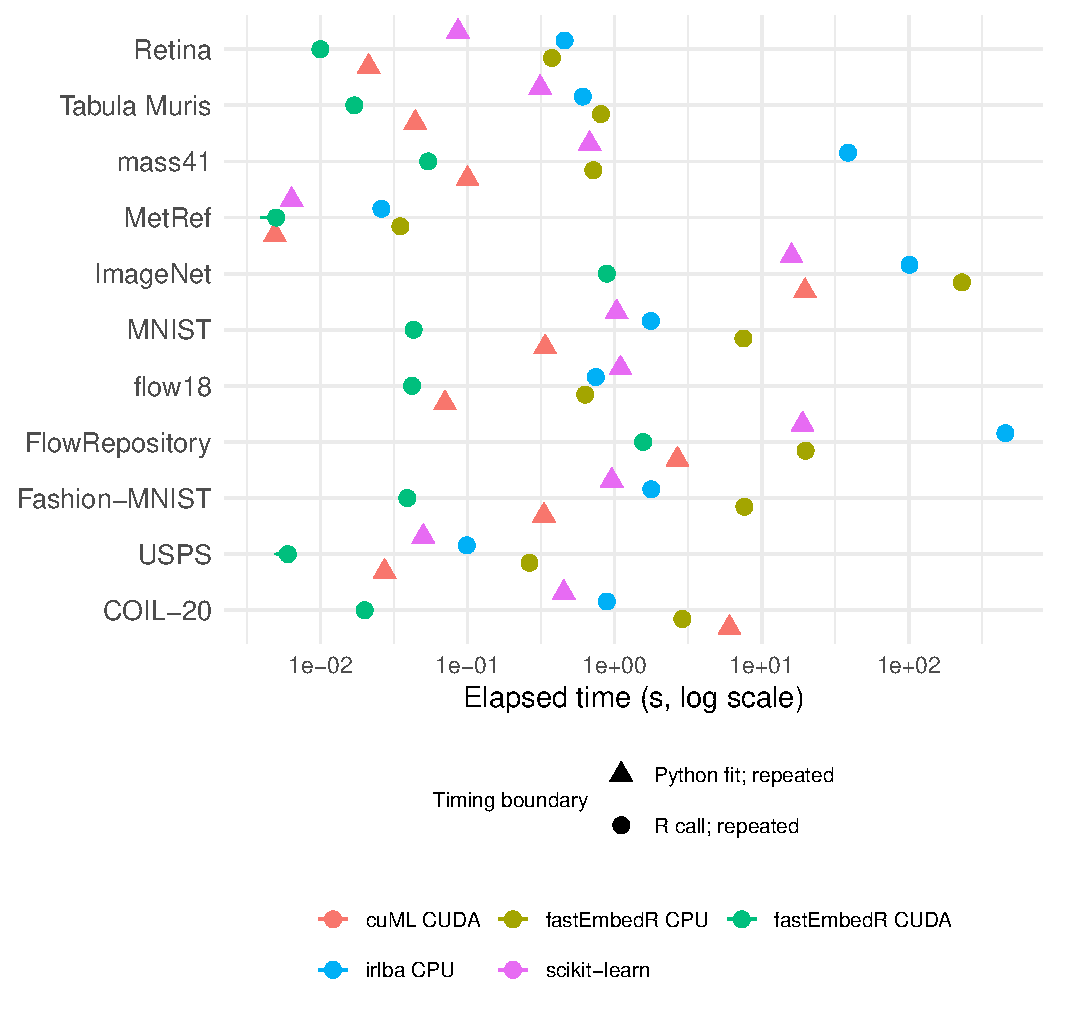
\includegraphics[width=0.98\textwidth]{figures/diagnostic_runtime_pca.pdf}
\caption{Observed PCA elapsed times in diagnostic campaign
  20260930T203319Z. Circles denote complete R public calls and triangles
  direct Python fits; filled markers have five same-seed repetitions and
  hollow markers show a completed single fit. Both scopes share an axis
  for inventory, not for a cross-scope speed ratio. Missing results and
  failures are identified in Supplementary Table~S1.}
\label{fig:diagnostic-runtime-pca}
\end{figure}

\begin{figure}[!t]
\centering
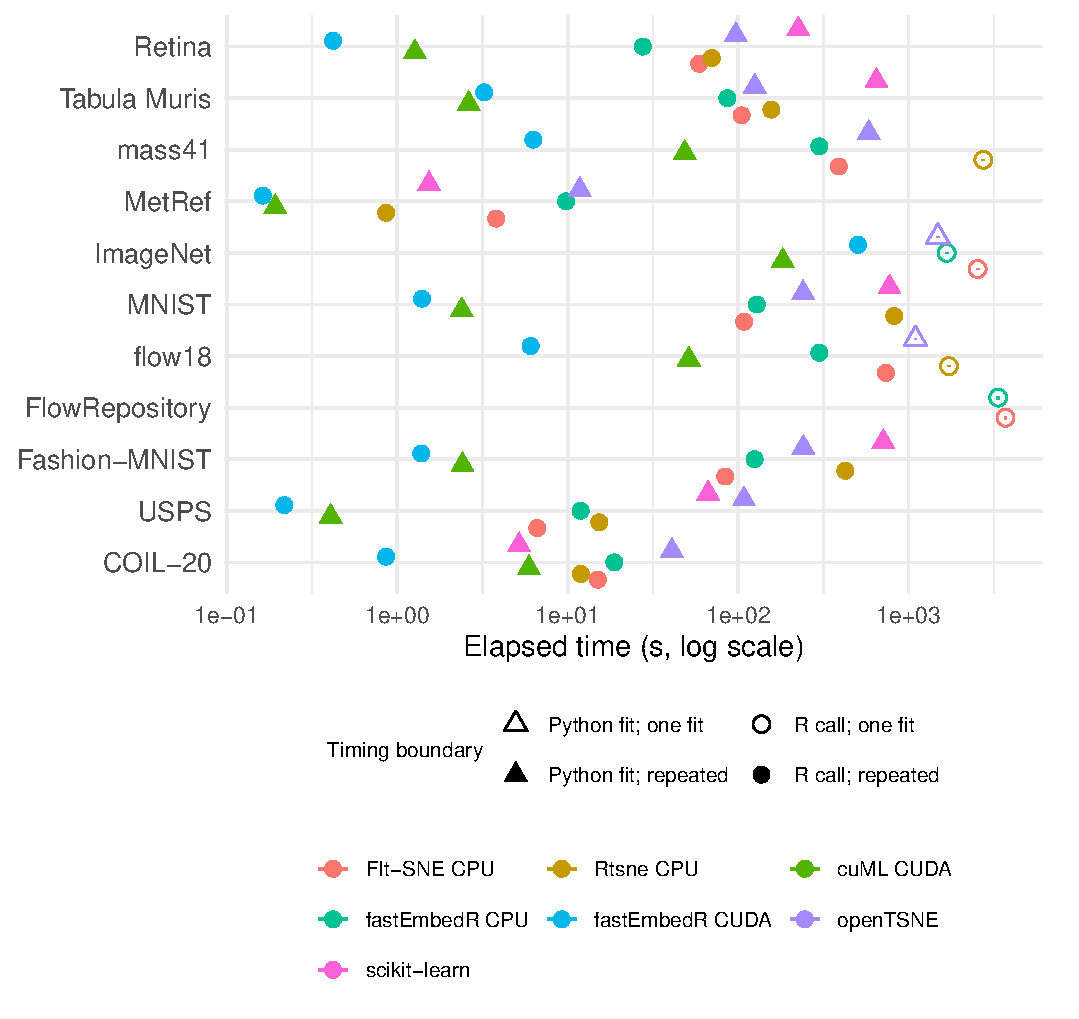
\includegraphics[width=0.98\textwidth]{figures/diagnostic_runtime_tsne.pdf}
\caption{Observed two-dimensional t-SNE elapsed times in the same
  full-data diagnostic campaign. R public-call and direct-Python fit
  measurements appear together but have distinct marker shapes and are
  not directly comparable. Hollow markers indicate completed single fits;
  missing results are coded in Supplementary Table~S1.}
\label{fig:diagnostic-runtime-tsne}
\end{figure}

\begin{figure}[!t]
\centering
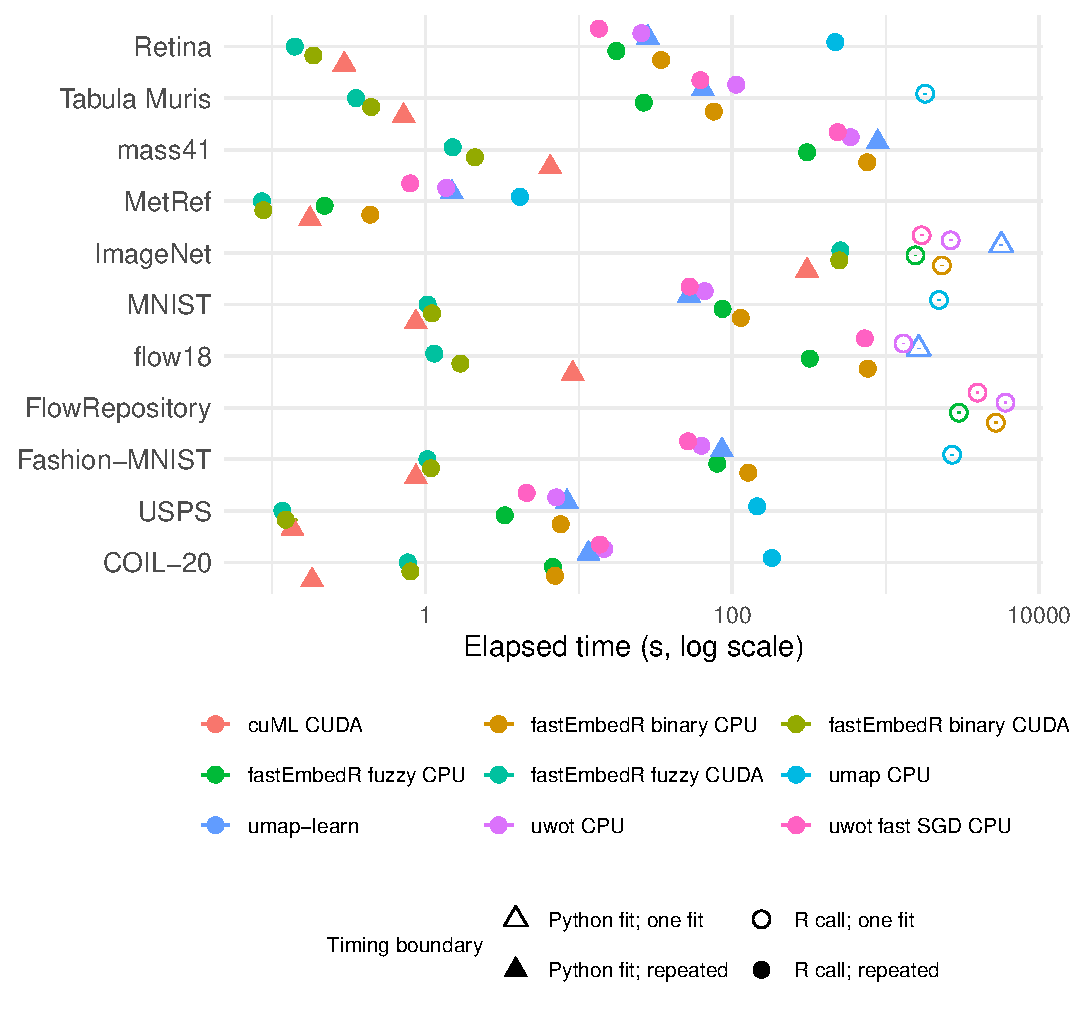
\includegraphics[width=0.98\textwidth]{figures/diagnostic_runtime_umap.pdf}
\caption{Observed two-dimensional UMAP elapsed times in the same
  full-data diagnostic campaign. Fuzzy and secondary binary UMAP routes,
  R and Python methods, and completed single fits are included. Timing
  boundaries and missing-result codes follow
  Figure~\ref{fig:diagnostic-runtime-pca} and Supplementary Table~S1.}
\label{fig:diagnostic-runtime-umap}
\end{figure}
\clearpage

Peak host resident memory and sampled CUDA device-memory increases are
reported in Supplementary Table~S9. They cover the
complete worker, including preparation and quality assessment, rather than
the direct-Python fit-only boundary. Short GPU peaks may escape sampling.

The campaign used a 7,200-second per-method limit. Its final audit is
\texttt{FAIL}, with 34 failed or timed-out tasks across the campaign and
four output-audit failures. Supplementary Table~S1 distinguishes timeout,
memory limit, other failure, and completed single fit. Some CUDA memory
peaks were not sampled adequately; missing values remain missing rather
than zero. Publication-level timing claims remain unresolved.

ImageNet is treated primarily as a runtime and memory stress test. Every
workflow fit in this campaign used the complete source matrix; source and
fitted row counts are displayed in Table~\ref{tab:data}.

Observed recall@30 was measured against exact full-reference neighbors.
The CUDA routes reached at least 0.9982; the CPU ImageNet and retina HNSW
routes reached 0.9672 and 0.9831, below the target 0.99. These sampled
checks are diagnostic and cannot be attributed to the optimizer.

Diagnostic median host peak RSS across complete CPU comparator workers was
1.53 GiB for \fastEmbedR t-SNE and 1.50 GiB for fuzzy UMAP, compared with
1.38 GiB for \pkg{Rtsne} and 5.32 GiB for the R \pkg{umap} package.
Device-wide median incremental memory in sampled CUDA workers was
1.03 and 0.78 GiB for \fastEmbedR t-SNE and UMAP, versus 1.28 and
0.73 GiB for direct cuML fits. These are whole-worker and sampled-device
observations, not fit-only or process-level memory ratios.

Across the ten data sets with successful full-workflow CPU and CUDA fits,
median CUDA-minus-CPU trustworthiness differences were +0.0037 for t-SNE
and -0.0027 for fuzzy UMAP; Preserve@30 differences were +0.0020 and
-0.0058. These are paired quality observations, not proof of identical
objectives or trajectories. Dataset-level values and the CUDA/cuML
comparison are in Supplementary Tables~S3 and~S2, respectively.

\subsection{Compact-support sensitivity}

When t-SNE has exactly $P$ candidate neighbors, its requested perplexity
equals the maximum possible perplexity on that support. Conditional
probabilities therefore approach uniform weights; reducing support changes
the affinity objective, not only its computational cost. In an exact-neighbor
affinity diagnostic at $P=30$, the median normalized conditional entropy was
approximately 1.000 for $k=P$ and 0.761 for $k=3P$.

At $P=10$, 20, and 30, fixed-neighbor sensitivity experiments generally
favored compact support for runtime and neighborhood preservation, whereas
wider support produced lower sampled KL for its different affinity objective.
The paired data-set counts and iteration budget are given in Supplementary
Table~S4; these calls are not complete workflows.

\subsection{Multicore scaling}

On COIL20, MNIST, flow18, and ImageNet, four CPU threads gave median
full-workflow speedups of 2.24 for t-SNE and 2.26 for fuzzy UMAP over one
thread. Scaling was not monotonic across 1, 2, 4, 8, and 12 threads; stage
times and per-data-set efficiency appear in Supplementary
Table~S5.

\subsection{Apple Metal}

The Apple M3 study covered MetRef, COIL20, USPS, MNIST, Fashion-MNIST,
Macosko retina, and Tabula Muris, spanning 873--100,102 observations and
50--16,384 variables. Median four-thread CPU-to-Metal speedup was 2.63
(IQR 1.62--2.88) for compact-support t-SNE, 1.97 (1.08--3.04) for fuzzy UMAP,
and 3.35
(1.63--5.85) for binary UMAP. Median Metal-minus-CPU trustworthiness
differences were +0.0006, +0.0027, and +0.0010. These results establish
performance on Apple M3 only. Other Apple Silicon systems are compatibility
targets unless separately benchmarked; Intel Macs are not supported by the
native Metal backend.

\subsection{Landmarking and held-out transformation}

A stratified 80/20 held-out experiment covered all 11 data sets. Median
query-to-reference Preserve@30 was 0.371--0.374 for t-SNE and
0.343--0.351 for fuzzy UMAP across CPU and CUDA; the reference did not move.
This tests new observations, not reconstruction of omitted fit rows.
In the separate 20-percent landmark experiment, median landmark/full
runtime ratios were 0.41 and 0.77 for CPU/CUDA t-SNE, and 0.34 and 1.29 for
CPU/CUDA UMAP. Median host-RSS ratios were near or above one, so
landmarking was not a universal memory saving. Detailed quality and memory
results are in Supplementary Tables~S6 and~S7.

\subsection{Supporting PCA and graph utilities}

On fixed subsets of 11 data sets, CPU and CUDA rank-2 PCA scores had
median aligned agreement of 0.999972 and approximately 1.000000 with
dense centered singular value decomposition. CPU ImageNet was an outlier
(0.783 score correlation). The latest campaign completed the
stored-graph clustering comparison on only two data sets, so it does not
support a broad clustering-performance claim. PCA accuracy, clustering
denominators, and graph-construction scope are documented in Supplementary
Tables~S10 and~S11.

\section{Discussion}

\fastEmbedR demonstrates that a single \proglang{R} package can expose
multicore CPU, Apple Metal, and NVIDIA CUDA implementations of fuzzy UMAP and
compact-support interpolation-based t-SNE while maintaining one typed
interface. The strongest
engineering gains come from reusing sparse structures, using float32
throughout the numerical payload, avoiding repeated \proglang{R}-native
copies, retaining accelerator state, pooling temporary memory, and reducing
kernel and synchronization overhead. The package does not introduce a new
UMAP or t-SNE objective; its contribution is a native, validated, and
backend-aware implementation and workflow.

The full-data workflow campaign is insufficient for a release-level speed
claim. Its failed final audit, incomplete memory sampling, and mixed
R/Python timing boundaries preclude reliable cross-method ratios,
despite useful stage and quality observations. A workflow ratio
combines implementation, search policy, precision, initialization, and
hardware; it does not isolate optimizer speed. Complete R calls and
direct-Python fit times answer different questions and are not pooled.

Compact support reduces affinity storage and attractive-force work while
making conditional probabilities nearly uniform within each selected row.
The t-SNE timing results therefore characterize the stated compact-support
method, not an affinity-equivalent replacement for conventional wider-support
t-SNE. Practical neighborhood quality and KL are reported with runtime for
every valid paired data set.

The production payload uses float32, so trajectories need not reproduce a
float64 implementation exactly. Accelerator atomics prevent a fixed seed from
guaranteeing bitwise GPU reproducibility. Metal performance evidence is
currently limited to one Apple M3 system. Native GPU installation depends on
matching SDKs, compilers, drivers, linked libraries, and architecture flags.
The UMAP interface exposes scientifically central neighborhood, metric,
initialization, graph, backend, and seed controls but keeps several optimizer
parameters under a validated release policy. Landmarking can reduce CPU work
but is not guaranteed to accelerate a resident GPU pipeline or preserve local
quality on every data set. These constraints should guide method selection
and reporting.

The file-backed routes are experimental rather than part of the headline
workflow comparison. Bounded-memory component tests have processed inputs
larger than host RAM, but a converged full-data t-SNE and UMAP comparison
on a real beyond-RAM data set is not established here. Multi-GPU row
partitioning of PCA, search, or landmark projection does not demonstrate
a multi-GPU full embedding. Disk capacity and graph-construction time
remain important limits even when the input itself can be streamed.

Observed approximate-neighbor recall is another limitation. The lowest
CPU recall@30 was 0.9672 on full-source ImageNet, below the target 0.99.
Search recall is consequently reported beside embedding quality,
and no claim treats ImageNet CPU results as optimizer-only evidence. Strong
CPU scaling was also nonmonotonic: eight threads had higher median
total-workflow speedup than twelve across the measured data sets.

Backend-native PCA removes a separate preprocessing boundary and can return a
t-SNE-ready initialization. Optional graph clustering reuses a graph already
constructed for an embedding workflow, but remains logically separate from
evidence for UMAP or t-SNE correctness. Walktrap is most appropriate for
smaller graphs because its agglomerative stage is CPU-only and has a denser
working set than the multilevel Louvain and Leiden paths.

\section{Reproducibility, availability, and sustainability}

The \href{https://github.com/tkcaccia/fastEmbedR}{package source} is available
under the MIT license. An
\href{https://tkcaccia.github.io/fastEmbedR/}{online tutorial and function
reference} documents installation, backend selection, and principal workflows.
Questions and bug reports are handled through the public
\href{https://github.com/tkcaccia/fastEmbedR/issues}{issue tracker}.
Benchmark code, preprocessing instructions, environment recipes, parameter
manifests, and aggregation scripts are maintained in a separate
\href{https://github.com/tkcaccia/fastEmbedR-extra}{benchmark repository}.
Raw benchmark data, credentials, container images, and restricted inputs are
not redistributed.

The corrected campaign launcher records the package-source commit,
embedded source-tarball and container hashes, and benchmark-suite manifest.
It also records any container-build source patch; a Git commit alone is
insufficient to identify a patched installation. Campaign evidence includes
session information, compiler and linker
commands, hardware identity, seeds, parameters, input checksums, status for
every requested row, and repetition-level outputs. Public data are
reconstructed from their original sources with versioned scripts. Restricted
data must be obtained under the provider's terms; missing data produce an
explicit unavailable status rather than substitution.

The diagnostic campaign was \texttt{20260930T203319Z}, built from source
commit \texttt{7f22c52b} with a recorded container-build patch. Its
complete source, archive, library, container, and
benchmark-suite SHA-256 identifiers are in Supplementary
Table~S12; comparator identities and
quality-sample row identifiers are in the machine-readable campaign.

Each campaign status inventory records its requested rows. Unsuccessful
combinations remain explicit in the machine-readable archives; no speedup
ratio is reported as a release-level result from the failed campaign.

The package test suite covers public R behavior and portable native code.
Strict hardware jobs verify requested-versus-observed backend identity and run
PCA, neighbor search, matrix-input and precomputed-KNN UMAP and t-SNE,
held-out landmark projection, graph clustering, and numerical checks on real
Metal and CUDA hardware. CPU checks run on macOS, Linux, and Windows.
Hardware logs, source packages, binaries, and SHA-256 manifests accompany the
benchmark evidence. The replication bundle includes a small deterministic
\code{iris} script that completes on a standard CPU and separate instructions
for the large hardware benchmark.

Host-side line coverage is reported separately for R and portable native
code. Metal and CUDA device kernels are not credited by host instrumentation;
their current evidence consists of strict real-device execution and numerical
tests. Device-aware Metal and CUDA kernel coverage is consequently reported as
not measured rather than inferred from host-side bridge execution.

\section{Conclusion}

\fastEmbedR provides native float32 UMAP and compact-support
interpolation-based t-SNE for
multicore CPU, Apple Metal, and NVIDIA CUDA execution from \proglang{R}. Its
matrix, reusable-neighbor, PCA, landmark, transformation, graph-construction,
and community-detection interfaces share strict backend reporting and typed
metadata. Metal performance evidence is specific to the tested Apple M3
system and is not generalized to all Apple Silicon hardware. Numerical tests
support CPU and CUDA PCA projections, graph construction, clustering,
affinities, forces, and backend-specific optimization; a separate M3 study
supports the Metal route on that system. The diagnostic campaign does not
establish release-level runtime reductions. The CPU
ImageNet PCA and HNSW-recall outliers show why data-set-level diagnostics must
accompany aggregate summaries.

\section*{Acknowledgments}

The authors thank the University of Cape Town ICTS High Performance Computing
team for providing a high-performance computing facility for this study
(\url{https://ucthpc.uct.ac.za/}).

\bibliography{fastEmbedR_JSS}

\end{document}
